\documentclass[final]{beamer}
\usepackage{beamerposter}
\usepackage{booktabs}
\usepackage{amssymb}
\usepackage{listings}
\usepackage{courier}
\usepackage{float}
\usepackage{graphicx}
\usepackage{caption}
\usepackage{fontawesome}
\usepackage[scale=1]{ccicons}
\usepackage{hyperref}
\usepackage[backend=biber,sorting=anyt,style=numeric]{biblatex}
\addbibresource{refs.bib}

% lorem ipsum packages
\usepackage[english]{babel}
\usepackage{blindtext}
\usepackage{lipsum}


% custom commands
\newcommand{\code}[1]{\texttt{#1}}


% styling commands - template from http://www.latextemplates.com/cat/conference-posters
\usetheme{confposter}
% \setbeamercolor{}{}
\usefonttheme{professionalfonts}
\setbeamerfont{block body}{series=\sffamily, size={\fontsize{32}{36}}}
\addtobeamertemplate{block end}{}{\vspace*{4ex}} % White space under blocks
\addtobeamertemplate{block alerted end}{}{\vspace*{4ex}} % White space under highlighted (alert) blocks


% layout
% 4-column layout, separation width = 0.04 of paper width
% onecolwid = (1-((4+1)*sepwid))/4
% twocolwid = (2*onecolwid)+sepwid
\newlength{\sepwid}
\newlength{\onecolwid}
\newlength{\twocolwid}
\setlength{\sepwid}{0.02\paperwidth} % Separation width (white space) between columns
\setlength{\onecolwid}{0.225\paperwidth} % Width of one column
\setlength{\twocolwid}{0.47\paperwidth} % Width of two columns
\setlength{\topmargin}{-0.5in} % Reduce the top margin size
\renewcommand*{\bibfont}{\footnotesize}


% document metadata
\title{Visualizing Mobile Phone Sensor Data in an R Environment}
\author{Riccardo Miccini}
\institute{Technical University of Denmark - DTU}
\date{\today}


% begin document - single frame, multi-column layout
\begin{document}
\begin{frame}[t]
\begin{columns}[t]

% column 1 - left
\begin{column}{\onecolwid}
	% objectives
	\begin{alertblock}{Objectives}
		The aim of the project is the application of methods for visualizing mobile phone (Android, iPhone) sensor measurements in an R environment, using the \emph{Google Cloud} as buffer.
		The system has to be able to:
		\begin{itemize}
			\item Collect GPS positioning data from mobile phones and store them remotely.
			\item Read the content of the spreadsheet from an R environment in real-time, and visualize spatial data on a map and other information on plots.
			\item Allow the user to interact with the data - filtering, zooming, scrolling, exporting\dots
		\end{itemize}
	\end{alertblock}

	% intro
	\begin{block}{\faCommenting \, Introduction}
		The project has been carried out under the supervision of profs. John Aasted S{\o}rensen and Ian Bridgwood, as part of a multidisciplinary project.

		The implemented system is composed of three main elements: a series of end users' mobile devices, a remote host, and a \emph{data analyst} station.
		The former are equipped with a custom-made application capable of submitting GPS data to a remote \emph{Google Sheet} document, which acts as a database and is accessible through the cloud.
		The data analyst can then visualize the collected data in real-time, using the provided R scripts and a web browser.

		\bigskip

		\emph{All brands, product names, logos, or other trademarks featured or referred to in this document are the property of their respective holders, and their use does not imply endorsement.}
	\end{block}

	% reqs
	\begin{block}{\faListUl \, Requirements}
		Here is a summarization of the functional and non-functional \emph{Software Requirements Specification}:
		\begin{itemize}
			\item The collected data shall include device ID, coordinates (latitude, longitude), altitude, speed, and timestamp.
			\item The mobile phone app shall submit data at a user-defined time interval.
			\item The R software shall visualize the spatial information using a map and any other data using a chart, in real-time.
			\item The user should be able to use the R application to filter and export the data.
			\item All the developed source code should be modular, reusable, and well-documented.
		\end{itemize}
	\end{block}
\end{column}

% column 2 - center
\begin{column}{\twocolwid}
	\begin{columns}[t, totalwidth=\twocolwid]
		% column 2.1 - centerleft
		\begin{column}{\onecolwid}\vspace{-.5in}
			% tools
			\begin{block}{\faWrench \, Tools}
				\textbf{Android Studio} is the official IDE for native Android development.
				It is distributed freely by Google for most platforms, and it is based on \emph{IntelliJ IDEA}, a proprietary Java development tool.
				It features:
				\begin{itemize}
					\item Code editor with completion and refactoring
					\item UIs designer, code generation wizards
					\item Integrated debugger and emulator
				\end{itemize}

				\vspace{.3in}
				\textbf{RStudio} is a free and open-source IDE for R, a language and software environment for statistical computing, data analysis, and visualization. The software comprises a text editor with code completion and syntax highlighting, an interactive command interpreter with built-in debug, command history, and data viewer.

				\vspace{.3in}
				The capabilities of R can be extended through a system of packages, which may provide graphics tools, statistical and data handling functions, or software bindings and APIs.
				\textbf{Shiny} is a framework for building live web applications in R. It comprises control widgets and graphic outputs, and uses a reactive model for determining which parts of the pages needs updating.
				Other used packages are:
				\begin{description}
					\item[\code{leaflet}] Maps service with custom overlays
					\item[\code{plotly}] Interactive and customizable plotting engine
					\item[\code{googlesheets}] Wrapper for the \emph{Google Sheets} APIs
					\item[\code{dplyr}] Functions for manipulating data
				\end{description}
			\end{block}
		\end{column}

		% column 2.2 - centerright
		\begin{column}{\onecolwid}\vspace{-.5in}
			% implementation
			\begin{block}{\faCode \, Implementation}
				%The project required the following software to be developed:
				%\begin{itemize}
				%	\item A mobile phone App
				%	\item An R Shiny web application
				%\end{itemize}

				%\begin{figure}
				%	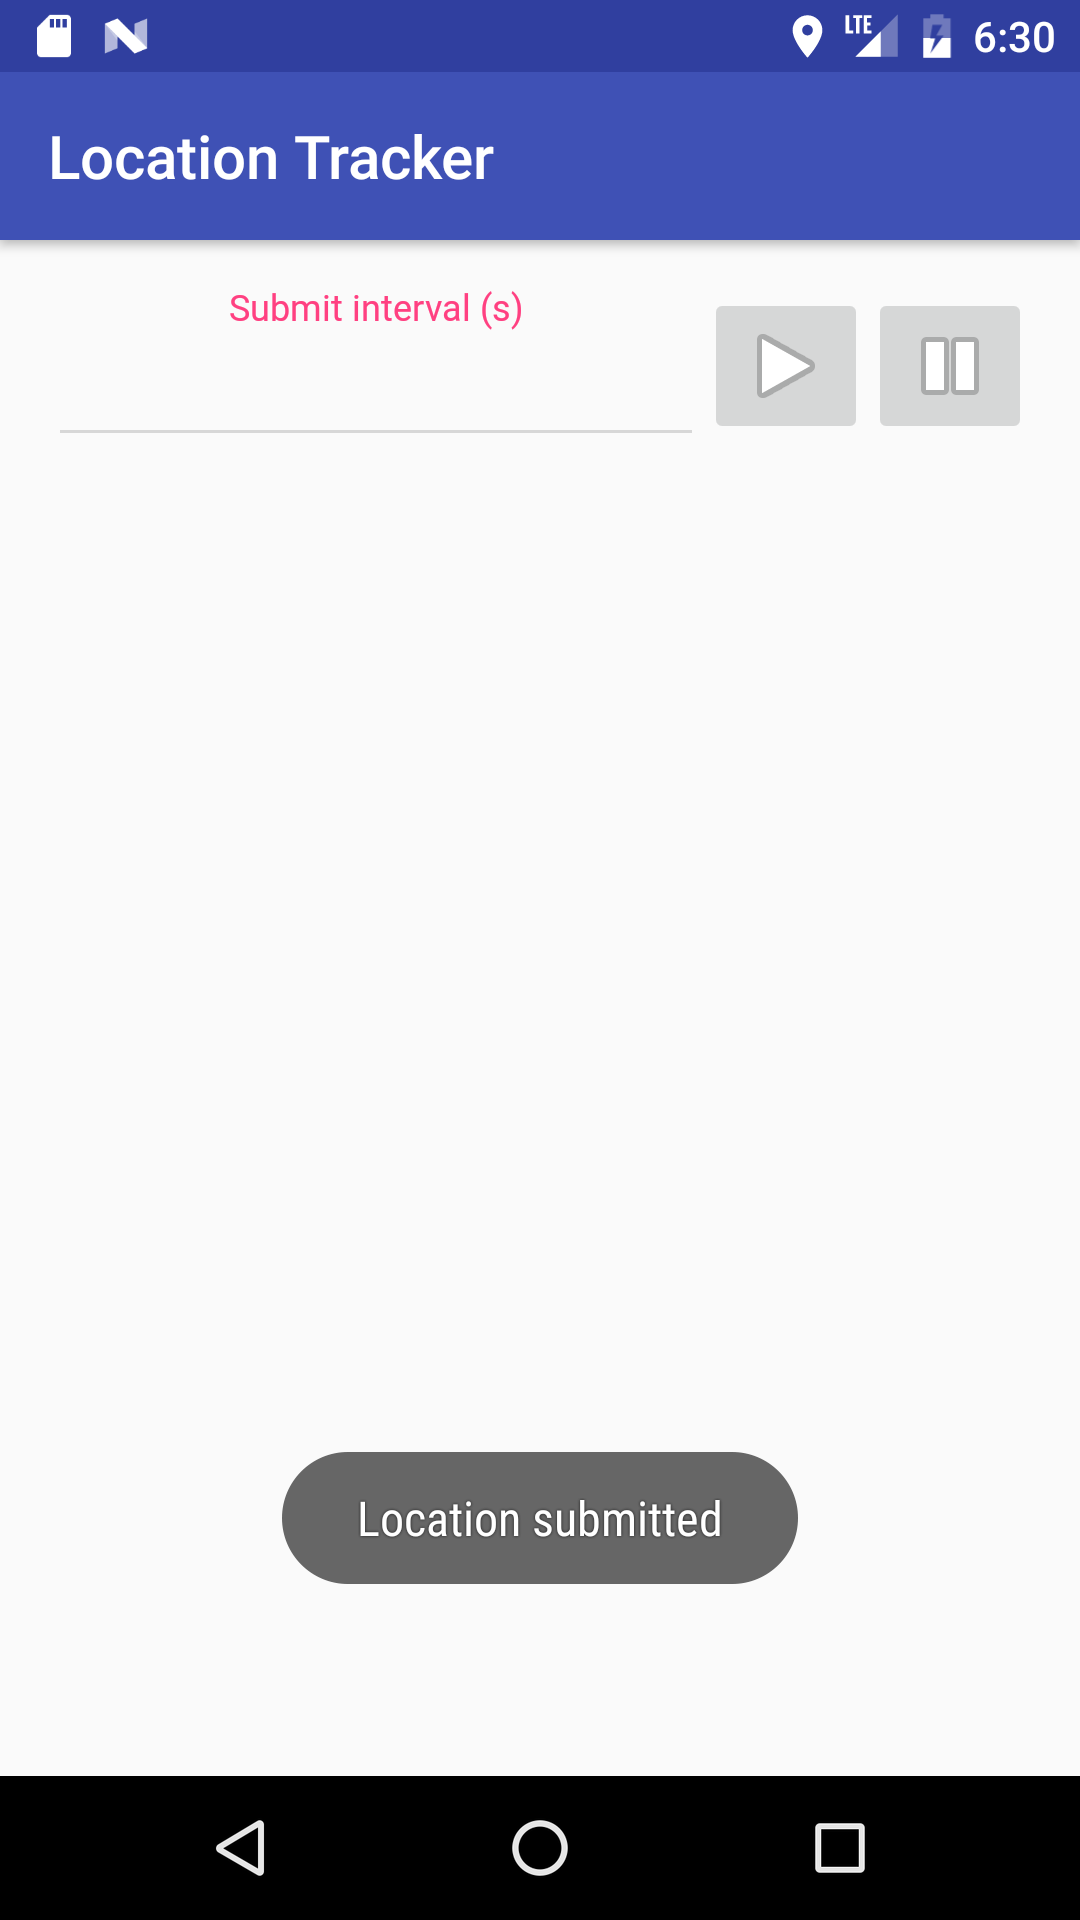
\includegraphics[width=0.25\onecolwid]{ss_app.png}
				%\end{figure}
				\begin{figure}
					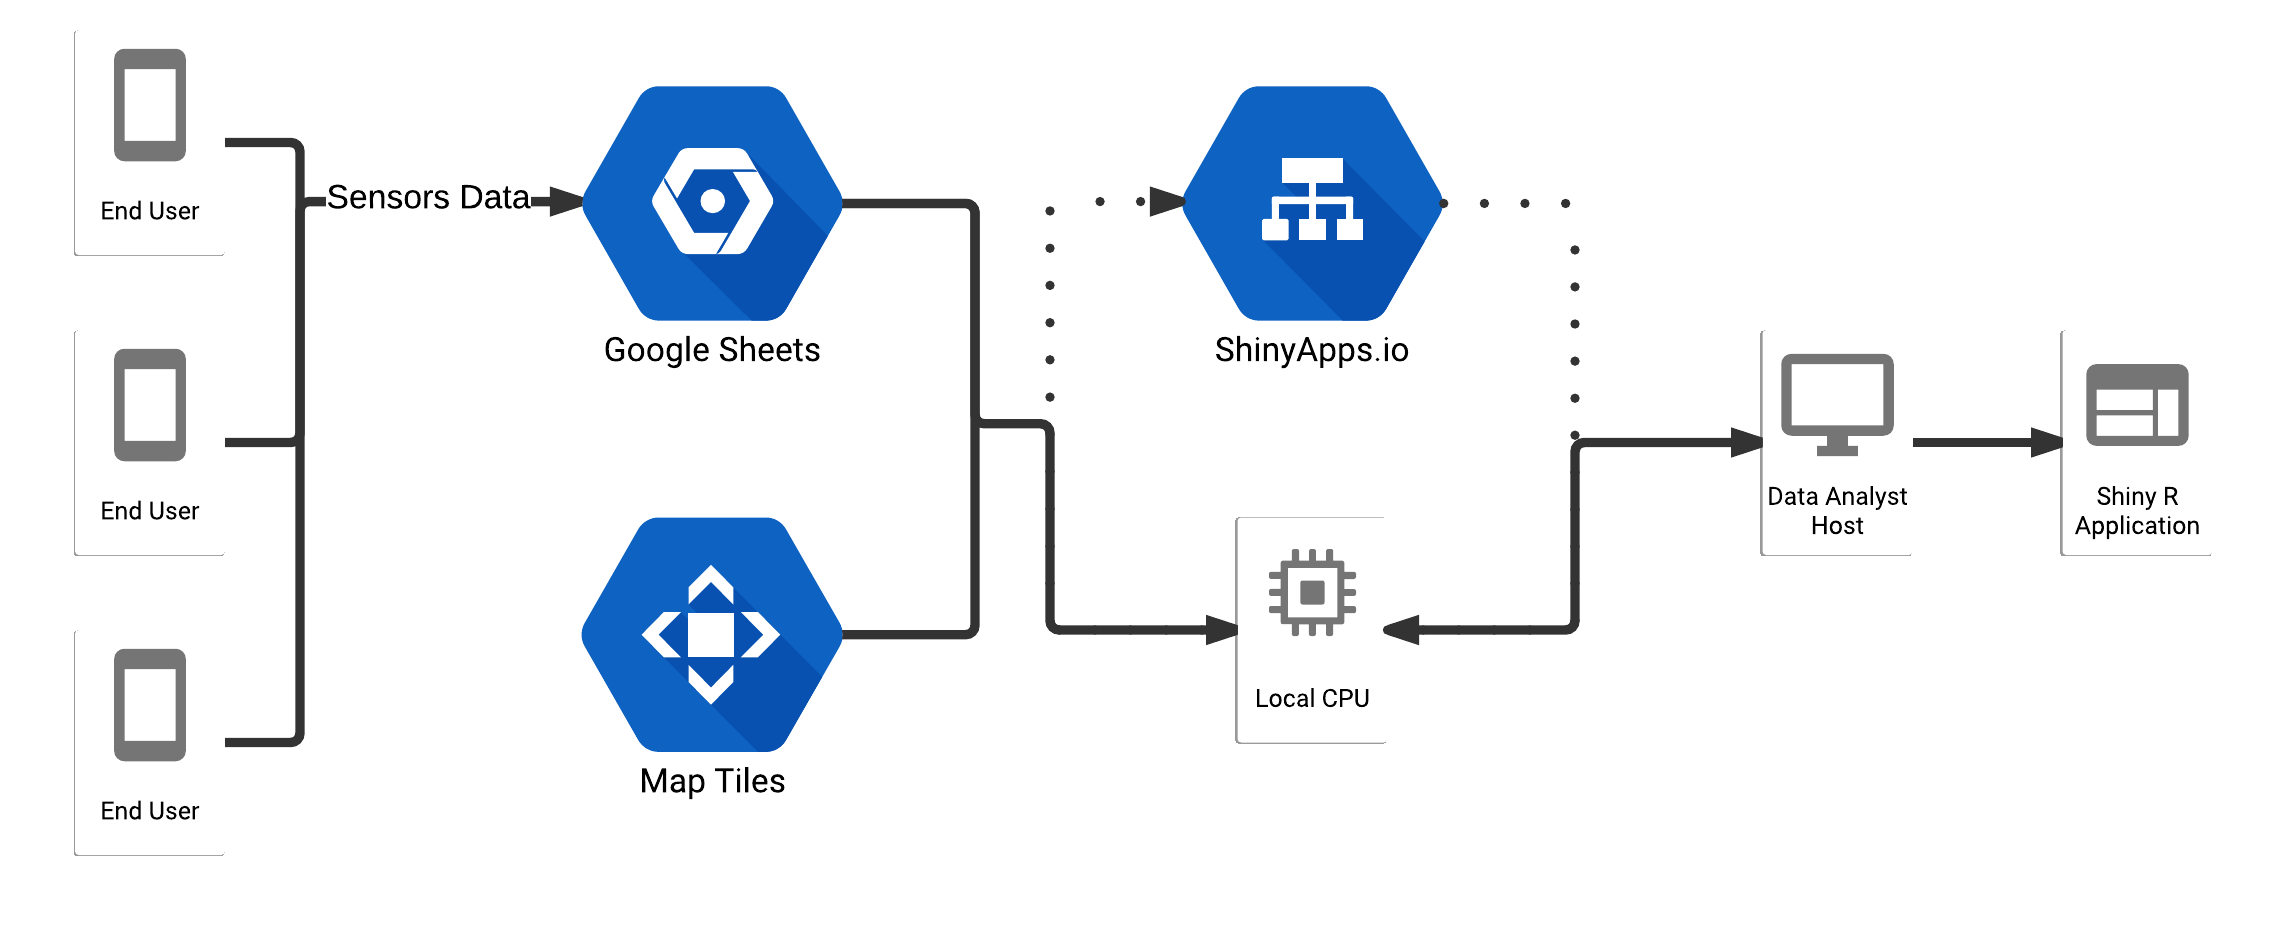
\includegraphics[width=0.8\onecolwid]{block_dia.png}
					\caption{Overall system infrastructure: network diagram}
				\end{figure}

				The \textbf{phone app} is responsible for collecting the GPS data and submitting them to the remote storage location, provided by \emph{Google Sheets}.
				Sheets is accessed through its APIs that allows third-party applications to manipulate and manage documents.
				The Android version of the app has been developed in JAVA using the \emph{Android Studio} environment and the \emph{Android SDK} libraries.
				A corresponding \emph{iOS} application has also been developed, performing the same tasks as the Android version.


				\vspace{.3in}
				The \textbf{R application} takes care of gathering the data from the spreadsheet, filtering it, and visualizing it on a web UI composed of a map and chart.
				It is built around the \emph{Shiny} framework, is accessible through a web browser, and can be hosted remotely.
				The application is composed of a front-end script which specifies the layout and widget elements of the webpage, and a back-end script that periodically queries the Sheet document, filters its data according to the user input, and generates and shows the map overlays and plot.
			\end{block}
		\end{column}
	\end{columns}

	% main figure section
	\vspace{-1cm}
	\begin{figure}
		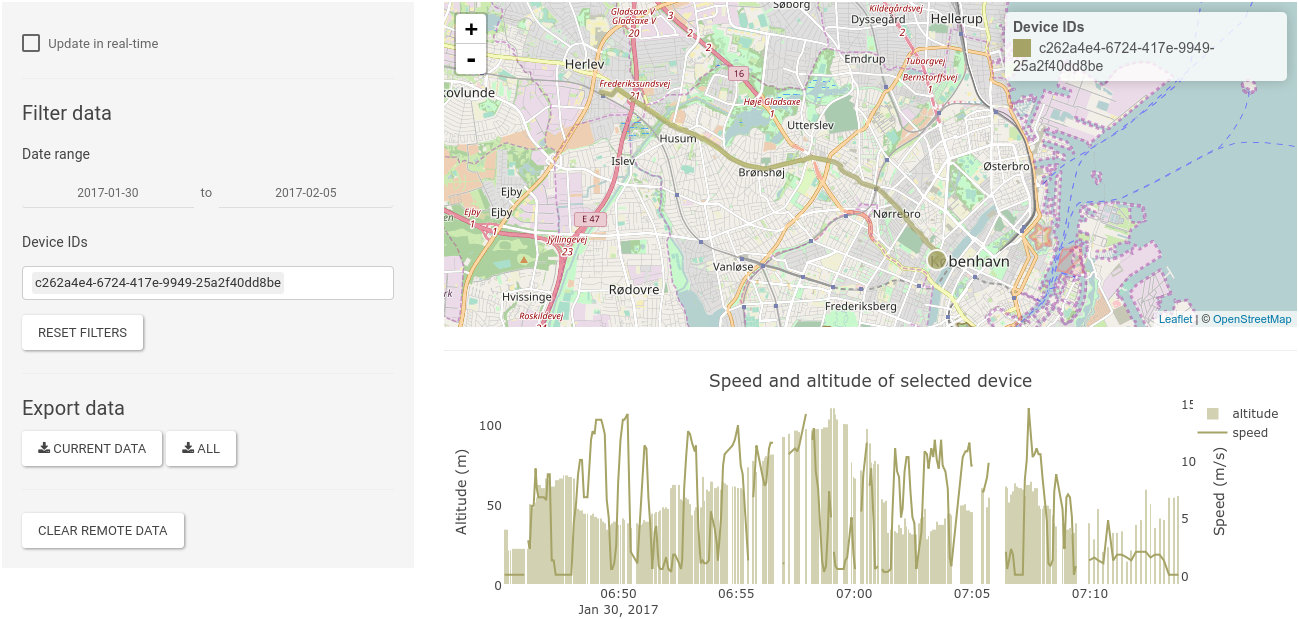
\includegraphics[width=\twocolwid]{ss_ui.png}
		% \caption{Figure caption}
	\end{figure}

	% copyright notice
	\vspace{2cm}
	\begin{center}
		{\small{This work is licensed under a \emph{Creative Commons Attribution-NoDerivatives 4.0} International License.}}\\
		\ccbynd
	\end{center}
\end{column}

% column 3 - right
\begin{column}{\onecolwid}
	% testing
	\begin{block}{\faCheckCircle \, Verification}
		The functionality of the developed solution has been verified by conducting \emph{acceptance testing}.
		The following tests have been performed and passed:
		\begin{itemize}
			\item Phone app
			\begin{itemize}
				\item Press button {\scriptsize\faPlay}
				\item Insert time interval, press button {\scriptsize\faPlay}
				\item Press button {\scriptsize\faPause}
				\item Verify content of the Google Sheets document
			\end{itemize}
			\item R Shiny appllication
			\begin{itemize}
				\item Load R application
				\item Use UI controls to select a single device
				\item Press button {\scriptsize\faDownload} \emph{all}, inspect the file
				\item Filter data, press button {\scriptsize\faDownload} \emph{current data}, inspect the file
			\end{itemize}
		\end{itemize}

		\vspace{.3in}
		The performances of using Google Sheets as storage back-end has been assessed by determining its network capacity, as well as the computational power required after each update.
		The devised test consists in an R script repeatedly querying data from the Google Sheets servers, with increasing numbers of rows.
	\end{block}

	% conclusion
	\begin{block}{\faPieChart \, Results and Conclusion}
		The project has reached a satisfactory level of completion.
		Nevertheless, the system is far from optimal and could still benefit from further development, in particular:
		\begin{itemize}
			\item Allow app to track data during background operation
			\item Improve R application responsiveness by limiting the amount of transmitted data
			\item Adopt a different storage back-end, e.g. Google \emph{BigQuery}
		\end{itemize}

		The project has been a compelling opportunity for exploring the Google Services ecosystem as well as the Android and R development environments.
	\end{block}

	% refs
	\begin{block}{\faPaperclip \, References}
		\nocite{*}
		\printbibliography
	\end{block}

	% contacts
	\begin{alertblock}{ Conctact Information}
		\faUser \, Riccardo Miccini \hfill \faGithub \, miccio-dk \\
		\faEnvelope \, s137345@student.dtu.dk \hfill \faLinkedin \, rimiccini
	\end{alertblock}

\end{column}

\end{columns}
\end{frame}
\end{document}
